\documentclass[12pt,a4paper]{article}
\usepackage{ctex}
\usepackage{amsmath, amssymb}
\usepackage{graphicx}
\usepackage{subcaption}
\usepackage{geometry}
\geometry{margin=1in}

\title{NPDE program 05 实验报告}
\author{刘行 PB22000150}
\date{\today}

\begin{document}
\maketitle

\section{问题描述}

考虑一维线性对流方程
\begin{equation*}
    u_t + u_x = 0,\qquad -\infty < x < \infty,\ t>0,
\end{equation*}
其初值条件为一个方波:
\begin{equation*}
u(x,0)=
\begin{cases}
1, & 0.4\le x \le 0.6,\\
0, & \text{otherwise}.
\end{cases}
\end{equation*}

本实验采用有限差分方法, 在区间 $[0,1]$ 上施加周期边界条件.
使用以下三种差分格式对该方程进行数值求解:

\begin{itemize}
    \item FTBS (Forward Time Backward Space, 上风格式)
    \item FTCS (Forward Time Central Space, 中心格式)
    \item Lax--Wendroff 二阶格式
\end{itemize}

并分别在 CFL 数
\[
r=\frac{\Delta t}{\Delta x} = 0.2,\ 0.8
\]
情况下, 对 $t=0.05,\ 0.2,\ 0.8,\ 3.2$ 时刻的数值解进行比较.

此外, 根据作业(2) 的要求, 对三种格式的耗散性与色散性进行分析, 并结合实验结果进行评价.

\section{数值方法与稳定性分析}

对流方程 $u_t+u_x=0$ 的离散化形式统一写为
\begin{equation*}
u_j^{n+1}=u_j^n - \lambda (D_x u)_j^n,\qquad \lambda=\frac{\Delta t}{\Delta x}.
\end{equation*}

\subsection{FTBS 格式 (上风格式)}

\begin{equation*}
    u_j^{n+1}
    =u_j^n - \lambda (u_j^n-u_{j-1}^n).
\end{equation*}

Von Neumann 模分析可得其稳定条件为
\[
0 < \lambda \le 1.
\]
FTBS 引入数值耗散, 使解的跳跃处变得平滑, 方波会被 ``涂抹''.

\subsection{FTCS 格式 (中心格式)}

\begin{equation*}
    u_j^{n+1}
    = u_j^n - \frac{\lambda}{2}(u_{j+1}^n-u_{j-1}^n).
\end{equation*}

对 $u_t + u_x = 0$, FTCS 的放大因子满足
\[
|G(\theta)|>1,\quad \theta\ne 0.
\]
因此该格式对本问题 \textbf{无条件不稳定}, 振荡会随时间指数增长.

\subsection{Lax--Wendroff 格式}

\begin{equation*}
    u_j^{n+1}
    = u_j^n
      - \frac{\lambda}{2}(u_{j+1}^n-u_{j-1}^n)
      + \frac{\lambda^2}{2}(u_{j+1}^n - 2u_j^n + u_{j-1}^n).
\end{equation*}

Lax--Wendroff 为二阶格式, 具有较低数值耗散, 但会产生数值色散, 使得在间断附近出现振荡 (Gibbs 现象).

\section{实验设置}

取区间 $[0,1]$, 周期边界条件. 空间步长
\[
\Delta x = 0.05
\]
对应 $J=20$. 时间步长根据
\[
\lambda = \frac{\Delta t}{\Delta x}=0.2,\ 0.8
\]
选择, 最终时间 $T=3.2$.
对三种格式分别计算以下时刻的解:

\[
t=0.05,\quad 0.2,\quad 0.8,\quad 3.2.
\]

\section{实验结果}

\subsection{CFL 数 $r=0.2$ 的结果}

\begin{figure}[ht]
    \centering
    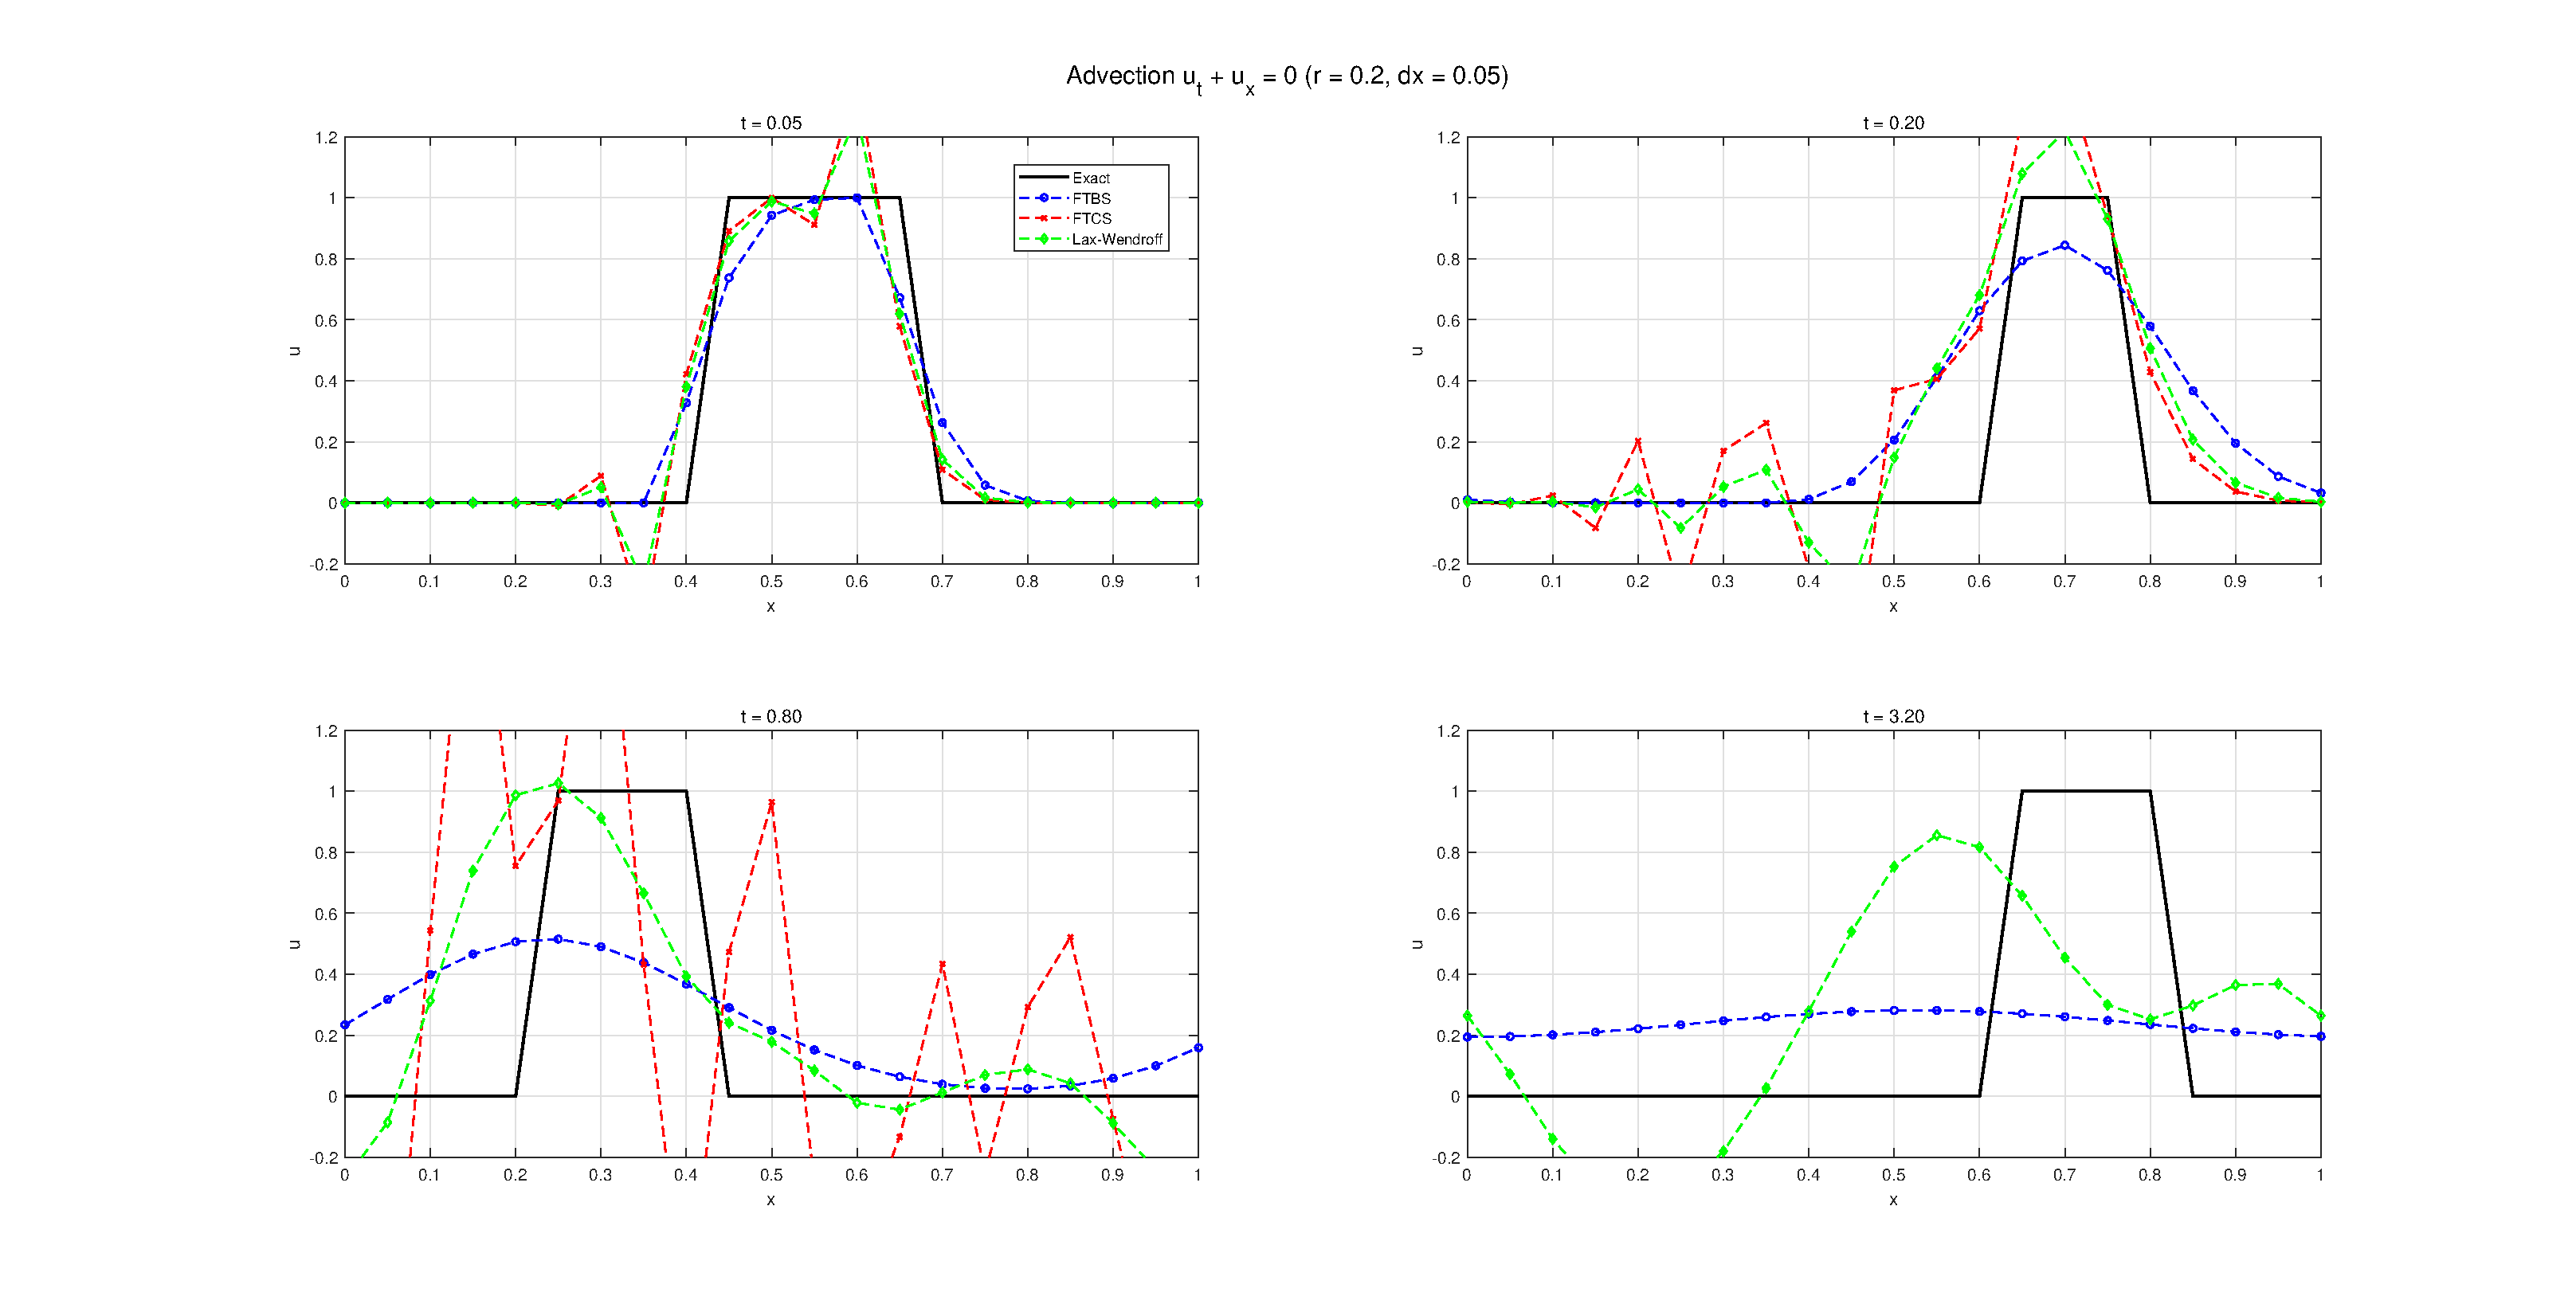
\includegraphics[width=0.9\textwidth]{fig/result_r0.2.eps}
    \caption{$r=0.2$ 时三种格式的数值解比较.
    \newline
    注意: FTCS 在 $t=3.20$ 时严重不稳定, 故未展示 (unstable/omitted).}
\end{figure}

\subsection{CFL 数 $r=0.8$ 的结果}

\begin{figure}[ht]
    \centering
    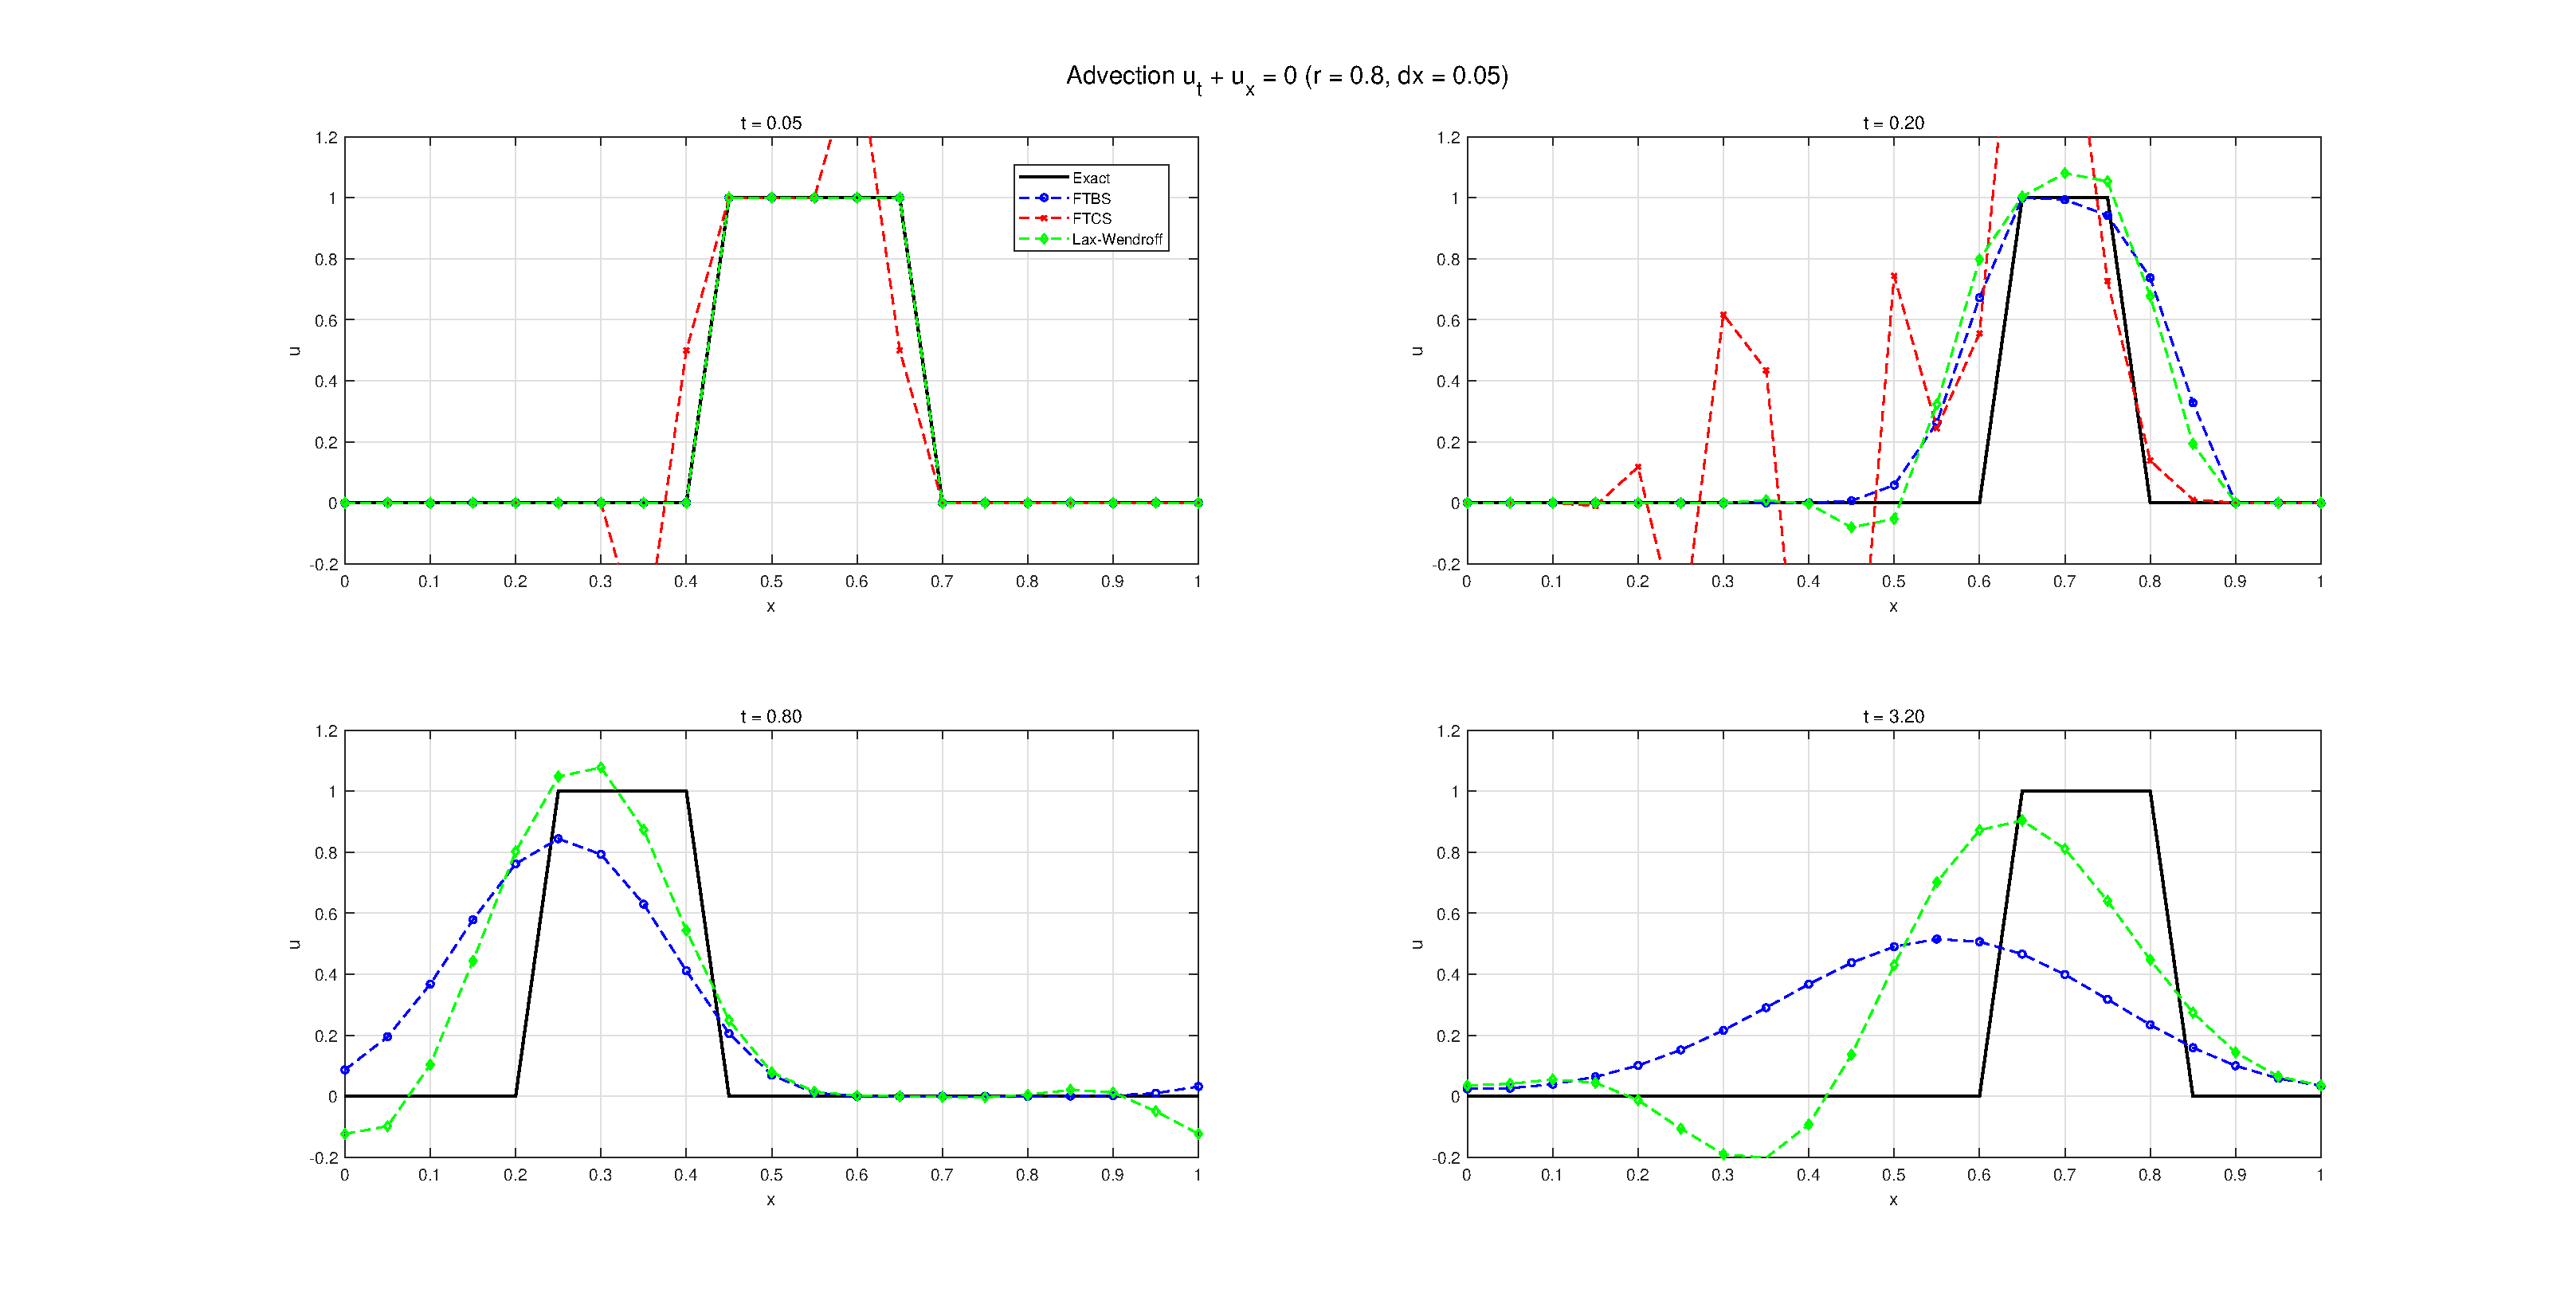
\includegraphics[width=0.9\textwidth]{fig/result_r0.8.eps}
    \caption{$r=0.8$ 时三种格式的数值解比较.
    \newline
    注意: FTCS 在 $t=0.80$ 与 $t=3.20$ 时严重不稳定, 故未展示 (unstable/omitted).}
\end{figure}

\section{结果分析与结论}

结合图像与理论分析, 可以得到以下结论:

\subsection*{(1) FTCS 的不稳定性}

FTCS 在本问题中无条件不稳定, 这是由其放大因子满足
\[
|G(\theta)|>1
\]
所决定的.
从实验可见:

\begin{itemize}
    \item $t=0.80, 3.20$ ($r=0.8$) 时振荡爆炸;
    \item $t=3.20$ ($r=0.2$) 也完全失稳.
\end{itemize}

因此图中未显示这些时刻.

\subsection*{(2) FTBS 的数值耗散 (dissipation)}

FTBS 虽然在 $0 < r \le 1$ 时稳定, 但具有强烈的数值黏性:

\begin{itemize}
    \item 方波边界被明显 ``涂抹'';
    \item $r=0.2$ 时耗散更强, 波形显著变钝;
    \item $r=0.8$ 时耗散较弱, 但仍可观察到锐利边界的退化.
\end{itemize}

\subsection*{(3) Lax--Wendroff 的数值色散 (dispersion)}

Lax--Wendroff 几乎不耗散, 保持了方波的高度与宽度, 但:

\begin{itemize}
    \item 在跳跃附近出现振荡 (ripple), 属于典型色散误差;
    \item 随时间推进振荡频率增高;
    \item 与 FTBS 相比, 整体波形保存得更好.
\end{itemize}

\subsection*{综合结论}

\begin{itemize}
    \item FTCS: 无条件不稳定, 不适用于对流方程.
    \item FTBS: 稳定但耗散强, 适合模拟稳定但模糊的传播.
    \item Lax--Wendroff: 二阶精度, 保持形状能力强, 但有色散振荡.
\end{itemize}

总体而言, 在本实验中:
\[
\text{FTBS 稳定但耗散} \quad \text{vs.} \quad
\text{Lax--Wendroff 稳定但色散}.
\]

对于具有间断的输运问题, 若要稳定且不过度抹平波形, Lax--Wendroff 通常优于 FTBS; 但在要求无振荡的场景中, FTBS 更为可靠.

\end{document}
